\section{Evaluation}\label{sec:evaluation}

We evaluate~\videojam{} in different scenarios and against the three baselines previously described. First, we compare it against Distream~\cite{zeng2020distream} to demonstrate the benefits of localized load balancing at function level, rather than a centralized approach for global load balancing. Next, we evaluate the system under different levels of loads to measure the performance of~\videojam{} as the workload increases. In addition, we test~\videojam{}'s ability to adapt to system configuration changes or failures, by subjecting it to critical situations such as the failure of a function or the failure of a node. Finally, we test the system's ability to deal with mobile cameras leaving and joining the architecture, demonstrating~\videojam{}'s ability to adapt to forecasting errors caused by sudden changes of video content.

\subsection{Comparison with Distream}
%In this experiment we compare~\videojam{} against a state-of-the-art video analytics architecture, Distream~\cite{zeng2020distream}. 
Distream's load balancing architecture is based on two main key concepts: the cross-camera workload and the partition point. The cross-camera workload determines the workload balance among cameras (also called ``Ends'') only. The partition point defines which functions of each pipeline are processed by Ends, while other functions are then executed on the server (called ``Edge''). The choice of offload proportion is handled in one of two different ways by the Ends: either a \textit{full-stochastic} (FS) or \textit{semi-stochastic} (SS) partitioning. In full-stochastic partitioning, the Ends generate a random partitioning proportion based on a Bernoulli random variable with probability set proportionally to the compute power of the Edge and End nodes. At every step of the pipeline, Ends draw a value from this variable and determine whether to process the function locally or offload it to the Edge. In semi-stochastic, the random value is drawn only at the partition point. In this case, the partition point is calculated as the point in the pipeline that evenly splits it proportionally to the compute power of the two components. 

\paragraph{\videojam{} outperforms baselines in heterogeneous deployments.} We compare~\videojam{} and other baselines in dealing with mixed traffic of mobile and fixed video cameras. To carry out this experiment, we deploy Distream using five \acrshort{gpu}-equipped nodes (as described in~\Cref{sec:implementation}). We deploy one instance of YOLO and one instance of OCR on each node, as required by Distream. We use the same five nodes for~\videojam{}, but we partition nodes hosting the pipeline for fixed and mobile cameras. In particular, we deploy two vehicle detection instances, three YOLOs, and five OCRs. We also deploy two other baselines, WRR and a~\videojam{} version that solely employs YOLOs for detection, and using the same configuration as~\videojam{}. Finally, we use four video sources, two mobile cameras and two fixed ones, draw randomly from the dataset presented in~\Cref{sec:implementation} and set to 20 frames per second. 

~\Cref{fig:distream_vs_videojam_heterogeneous} shows that~\videojam{} outperforms all other solutions, both in terms of response time, with 2.91$\times$ and 1.77$\times$ less response time compared to Distream's solutions, and reduces objects loss by 19\% and 4\%, respectively. This highlights the advantages of using a localized load balancing technique like~\videojam{}, and the limitation of approaches like Distream or a simplistic WRR. Further, the figure highlights that the use of mixed pipelines for different sources of traffic improves response time.  Indeed, the use of dedicated pipelines for fixed and mobile cameras, \ie, background substractor vs YOLO as explained~\Cref{sec:background_motivation}, improves classification performance incurring less load depending on the number of objects in each frame. Consequently, if the amount of objects in the video scene is low, no action, \ie, inference, will be taken, whereas detection techniques such as YOLO will take action even if no objects are present in the frames. This is supported by the performance improvement observed when comparing the two approaches on~\videojam{} (\ie, the one using vehicle detection over the one using only YOLOs). Furthermore, the results show that~\videojam{} has a response time 1.11$\times$
lower than~\videojam{} with YOLO only.

\begin{figure}
	\begin{minipage}[t]{.52\linewidth}
		\centering
		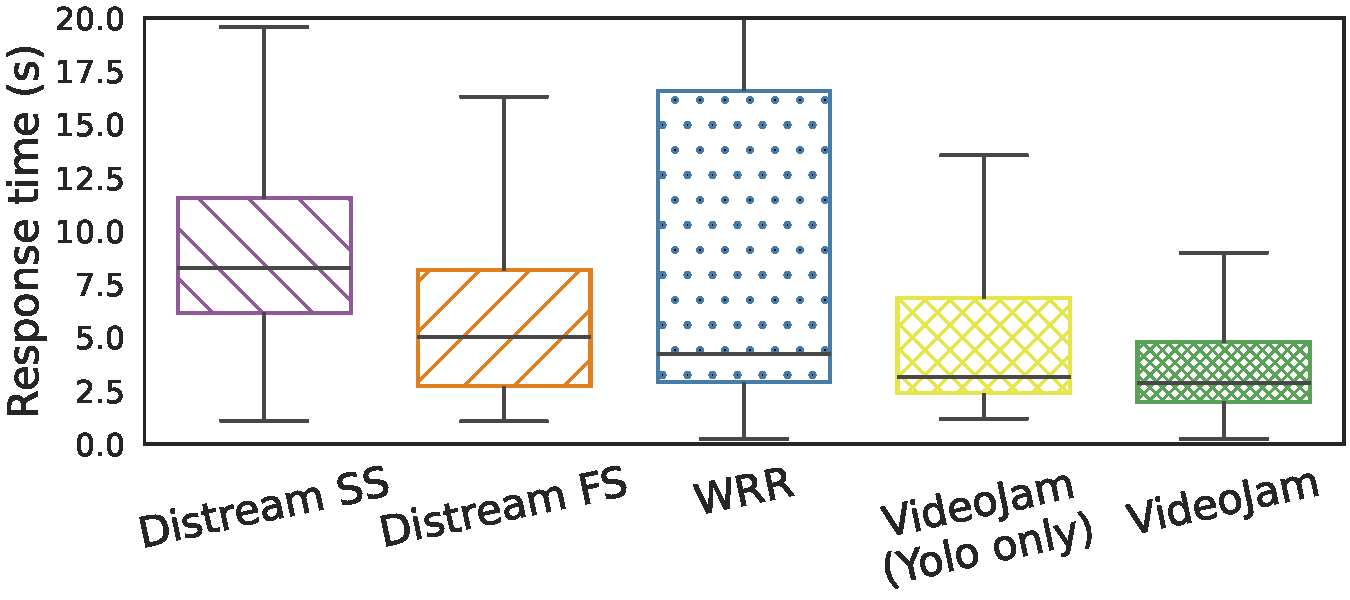
\includegraphics[width=\linewidth]{chapters/videojam/images/distream_vs_videojam/heterogeneous/response_time.pdf}
		\subcaption{Response time.}
	\end{minipage}
	\hfill
	\begin{minipage}[t]{.46\linewidth}
		\centering
		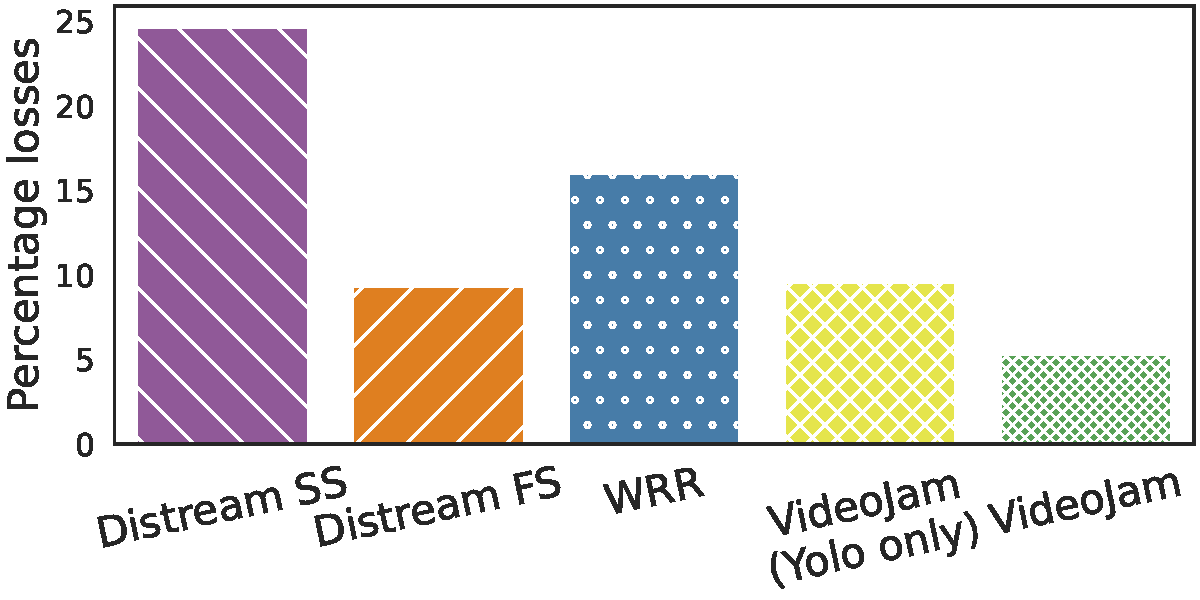
\includegraphics[width=\linewidth]{chapters/videojam/images/distream_vs_videojam/heterogeneous/percentage_losses.pdf}
		\subcaption{Percentage losses.}
	\end{minipage}
	\caption{Evaluation on a heterogeneous architecture shows a response time up to 2.91$\times$ lower than comparative approaches, and with fewer losses.}
	\label{fig:distream_vs_videojam_heterogeneous}
	\vspace{-3mm}
\end{figure}

\paragraph{\videojam{} outperforms Distream in mobile only scenarios.} In the previous experiment we have shown that~\videojam{} outperforms baselines when processing mixed types of video traffic. We now explore whether our solution can still outperform Distream when solely processing video traffic generated by mobile cameras. We do so to evaluate~\videojam{}'s load balancing technique, understanding whether the advantages presented previously are to be solely attributed to the use of different pipelines for different types of traffic or to the load balancing as well. In this experiment, we use the same experimental setup as in the previous experiment, the only difference being that we use YOLOs throughout the deployment for all baselines, and we use four mobile cameras.

~\Cref{fig:distream_vs_videojam} shows the performance of WRR, Distream, and~\videojam{}. We can observe that the semi-stochastic version of Distream incurs the worst performance in terms of both response time and loss: about 2.02$\times$ and 3.68$\times$, respectively, compared to~\videojam{}. Indeed, given the design of Distream, it is difficult to define the load balancing policy when considering the pipeline as a whole. In fact, two different functions (\eg, YOLO and OCR) on different nodes may become overloaded as traffic loads vary in time. This makes it very difficult to define an optimal load balancing policy for load distribution. Furthermore, in our observation, the considerable loss observed is due to the fact that a large portion of the video traffic remains continuously blocked in the Edge, which is unable to empty it quickly enough.

\begin{figure}
	\begin{minipage}[t]{.52\linewidth}
		\centering
		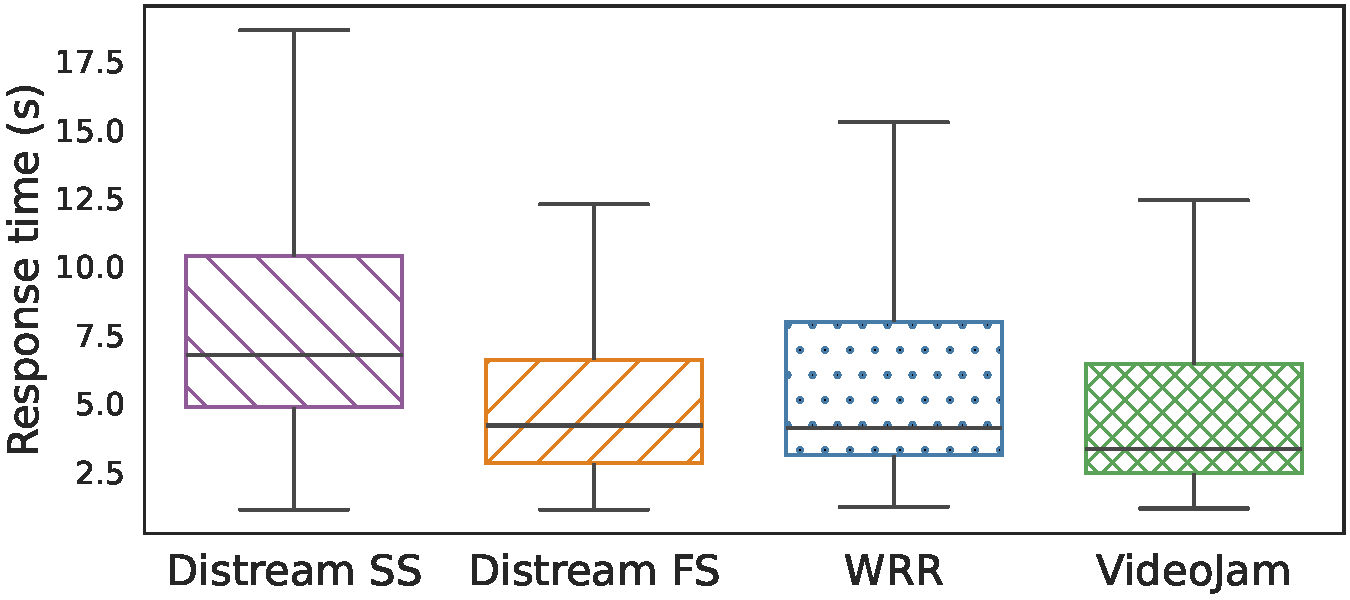
\includegraphics[width=\linewidth]{chapters/videojam/images/distream_vs_videojam/response_time.pdf}
		\subcaption{Response time.}
	\end{minipage}
	\hfill
	\begin{minipage}[t]{.46\linewidth}
		\centering
		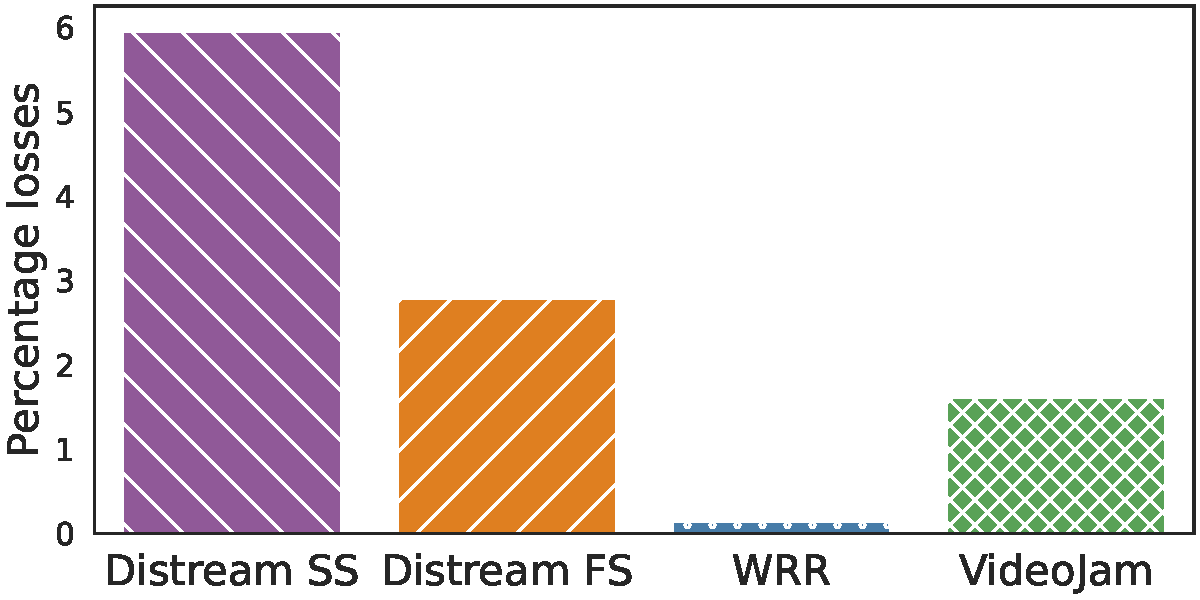
\includegraphics[width=\linewidth]{chapters/videojam/images/distream_vs_videojam/percentage_losses.pdf}
		\subcaption{Percentage losses.}
	\end{minipage}  
	\vspace{-1mm}
	\caption{Evaluation on mobile cameras shows that~\videojam{}'s response time is 1.25$\times$ shorter than Distream's.}
	\vspace{-3mm}
	\label{fig:distream_vs_videojam}
\end{figure}

Nevertheless, we observe similar response time results between the full-stochastic approach and~\videojam{}. The reason for this lies behind the simple offload policy implemented in this approach: as the pipeline consists of only two functions, the partition is only necessary at either YOLO or OCR, often leaving the Edge in charge of the full processing. Yet, this simplicity can incur increased loss, when these nodes become overloaded (about 3\% loss). We also observe that WRR experiences a lower percentage of loss compared to~\videojam{}. This is due to WRR's simpler load-balancing policy, which in some cases can be beneficial to loss, when frames spend more time being transmitted between nodes, slowing down the volume of traffic reaching the OCRs. In fact, we observe that WRR tends to balance load more aggressively across all available instances, thus increasing network usage (more details on this later in this section). Consequently, these frames are not queued fast enough to fill the ORC queues, explaining the small loss for WRR. This also explains the WRR's lower performance in terms of response time (1.22$\times$ lower response time than WRR). Ultimately, this shows that in certain instances, there might be a tradeoff to explore between response time and information loss. We leave this exploration for future work.



\paragraph{\videojam{} better handles node failures.} The aim of this experiment is to determine the impact of node failure on the performance of Distream, WRR, and~\videojam{}. To do this, we simulate two types of failure: the first is an End failure, the second an Edge failure.

~\Cref{fig:distream_vs_videojam_onfailure} summarizes the performance of each solution. We can observe a significant loss for Distream (about 15\% of the total traffic). The reason for this large loss is that after the Edge has failed, the last policy calculated by the Edge, \ie, the partitioning point, is still executed by the Ends and is not updated during the Edge's absence. So when the Edge comes back, the computation it is supposed to be dealing with since the last partition point update suddenly arrives, saturating the Edge in the process and causing several losses. Also, Distream's low response time is due to the fact that fewer frames are waiting in the queue to be processed after a large proportion of them have been lost.

Furthermore, we see the ability of~\videojam{} to be robust to failures and to react a recovery. Indeed, when a node failure occurs,~\videojam{} adapts the load balancing policy calculation to the available resources. When the failed node returns, the policy is recomputed and all the workload already accumulated is redistributed. This explains the low losses of around 2\% which are 6$\times$ lower than Distream's ones. WRR, on the other hand, does not present the same ability of robustness to failures, even though its policy is updated every time the system is stressed. And since its policy does not take into account the workload of the instances, the load previously accumulated during the downtime is not redistributed.

\begin{figure}
	\begin{minipage}[t]{.52\linewidth}
		\centering
		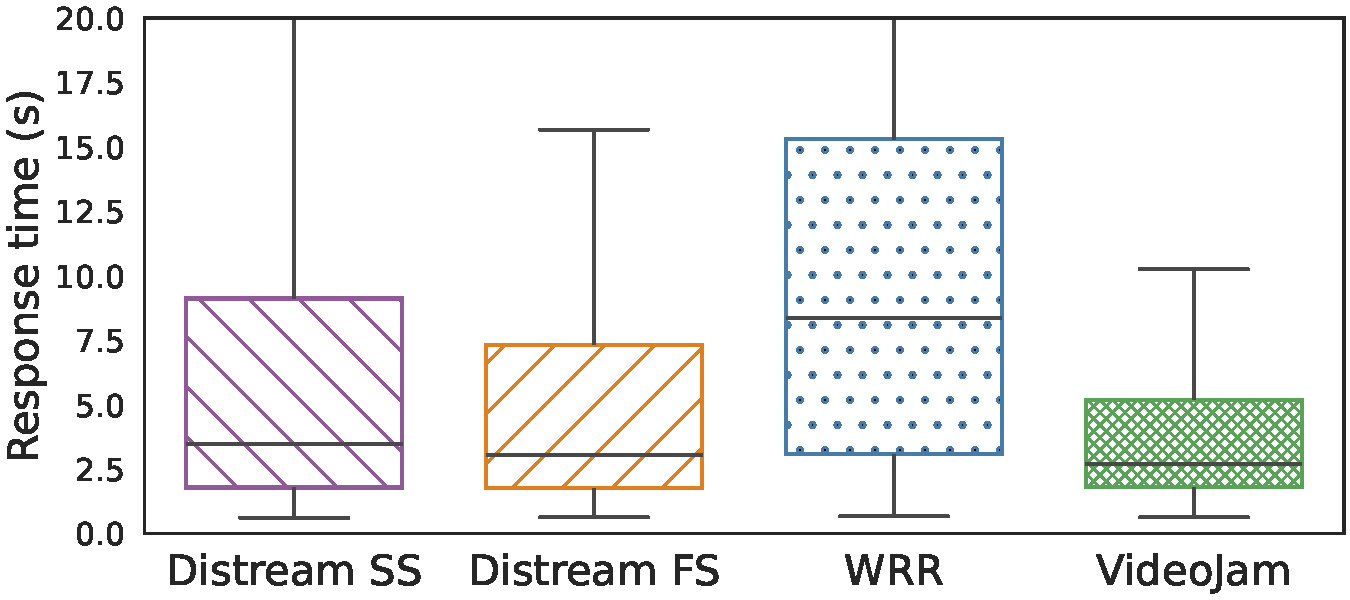
\includegraphics[width=\linewidth]{chapters/videojam/images/distream_vs_videojam/onfailure/response_time.pdf}
		\subcaption{Response time.}
	\end{minipage}
	\hfill
	\begin{minipage}[t]{.46\linewidth}
		\centering
		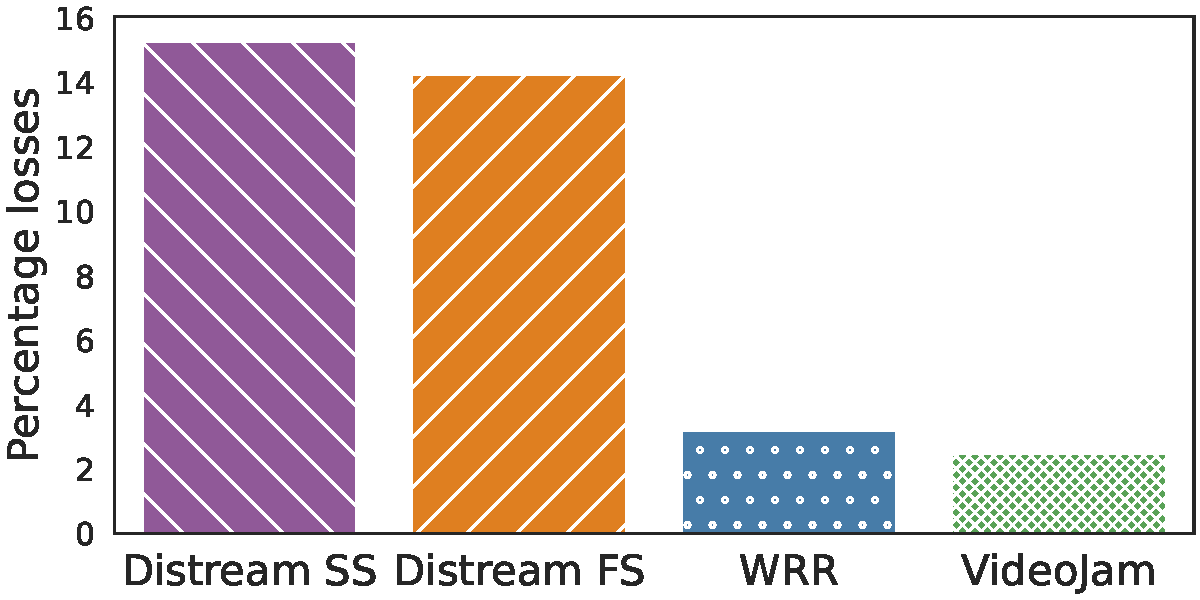
\includegraphics[width=\linewidth]{chapters/videojam/images/distream_vs_videojam/onfailure/percentage_losses.pdf}
		\subcaption{Percentage losses.}
	\end{minipage}
	\vspace{-1mm}
	\caption{Evaluation of Distream and~\videojam{} in the event of node failure, with the latter recording fewer losses while maintaining better response time.}
	\vspace{-3mm}
	\label{fig:distream_vs_videojam_onfailure}
\end{figure}



\subsection{Load Balancing Ablation Study}

In this section, we evaluate the effectiveness of~\videojam{}'s load balancing algorithm with respect to two alternative baselines, no load balancing and WRR.

\begin{figure*}[htb]
	\centering
	\begin{minipage}[t]{.3\linewidth}
		\centering
		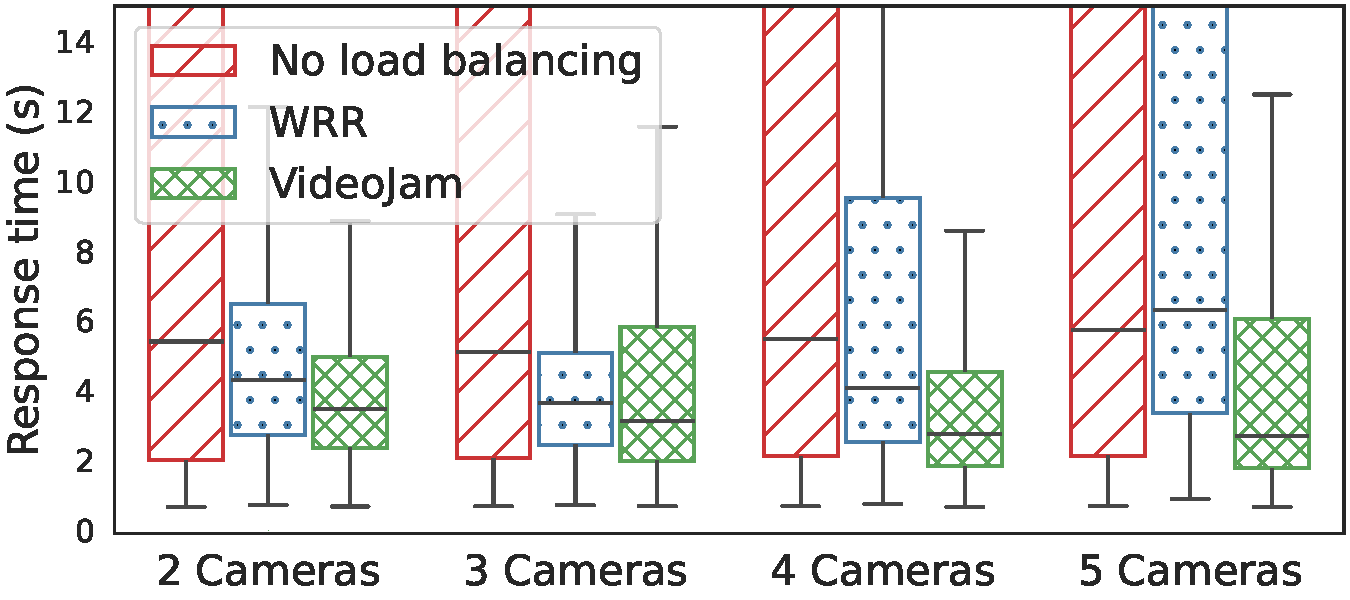
\includegraphics[width=\linewidth]{chapters/videojam/images/agains_weighted_roundrobin/response_time.pdf}
		\subcaption{Response time of the system.}
	\end{minipage}
	\hfill
	\begin{minipage}[t]{.3\linewidth}
		\centering
		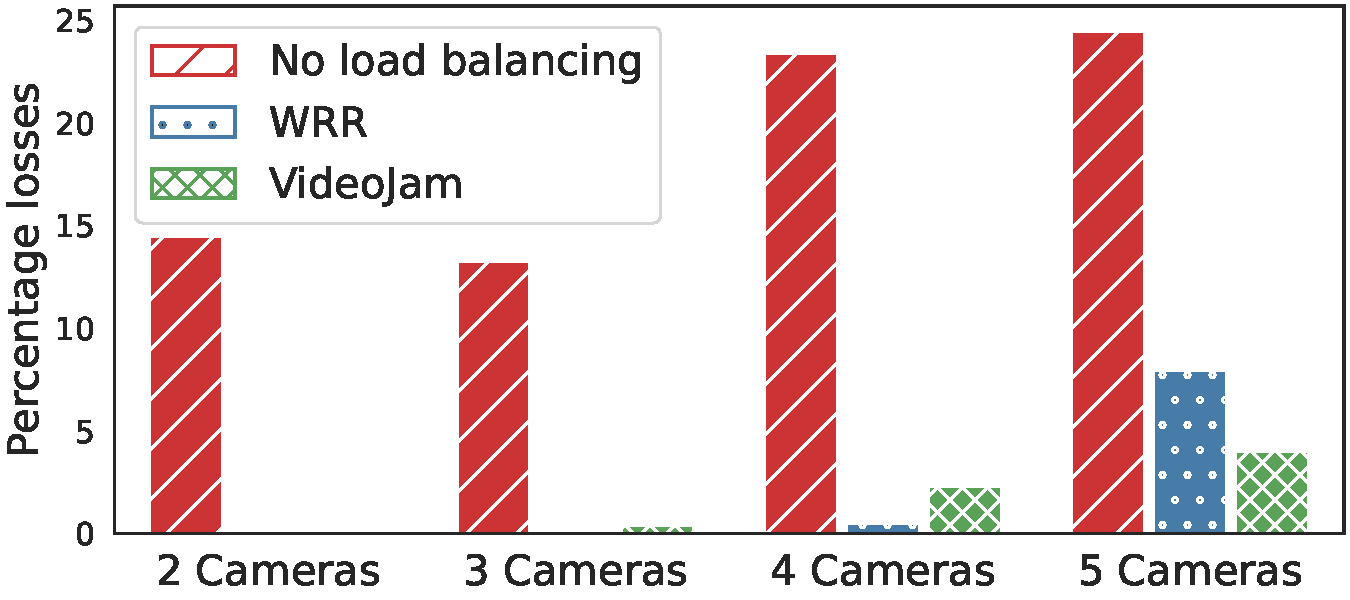
\includegraphics[width=\linewidth]{chapters/videojam/images/agains_weighted_roundrobin/percentage_losses.pdf}
		\subcaption{Percentage of frame lost.}
	\end{minipage}
	\hfill
	\begin{minipage}[t]{.3\linewidth}
		\centering
		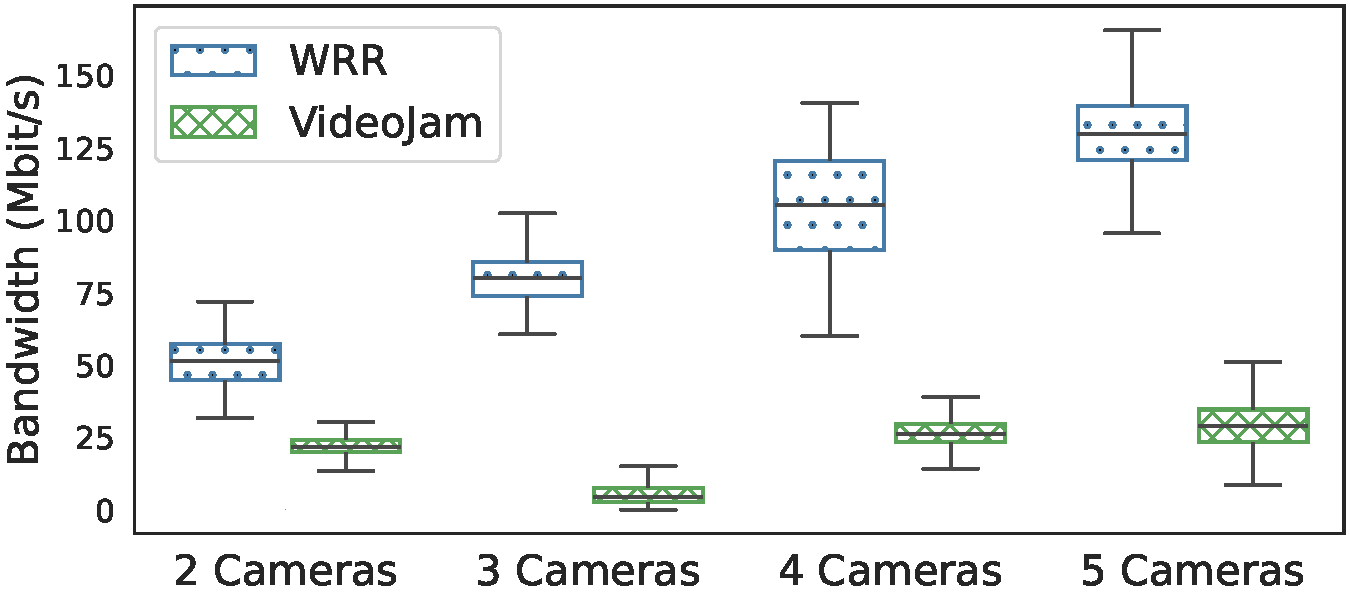
\includegraphics[width=\linewidth]{chapters/videojam/images/agains_weighted_roundrobin/bandwidth.pdf}
		\subcaption{Bandwidth used for offloading to neighbors.}
		\label{fig:against_wrr_bandwidth}
	\end{minipage}
	\vspace{-1mm}
	\caption{Evaluation on several configurations shows the need for a load-balancing technique and the effectiveness of~\videojam{} in achieving lower response times with less bandwidth usage.}
	\vspace{-3mm}
	\label{fig:against_wrr}
\end{figure*}

\begin{figure}[htb]
	\centering
	\begin{minipage}[t]{.66\linewidth}
		\centering
		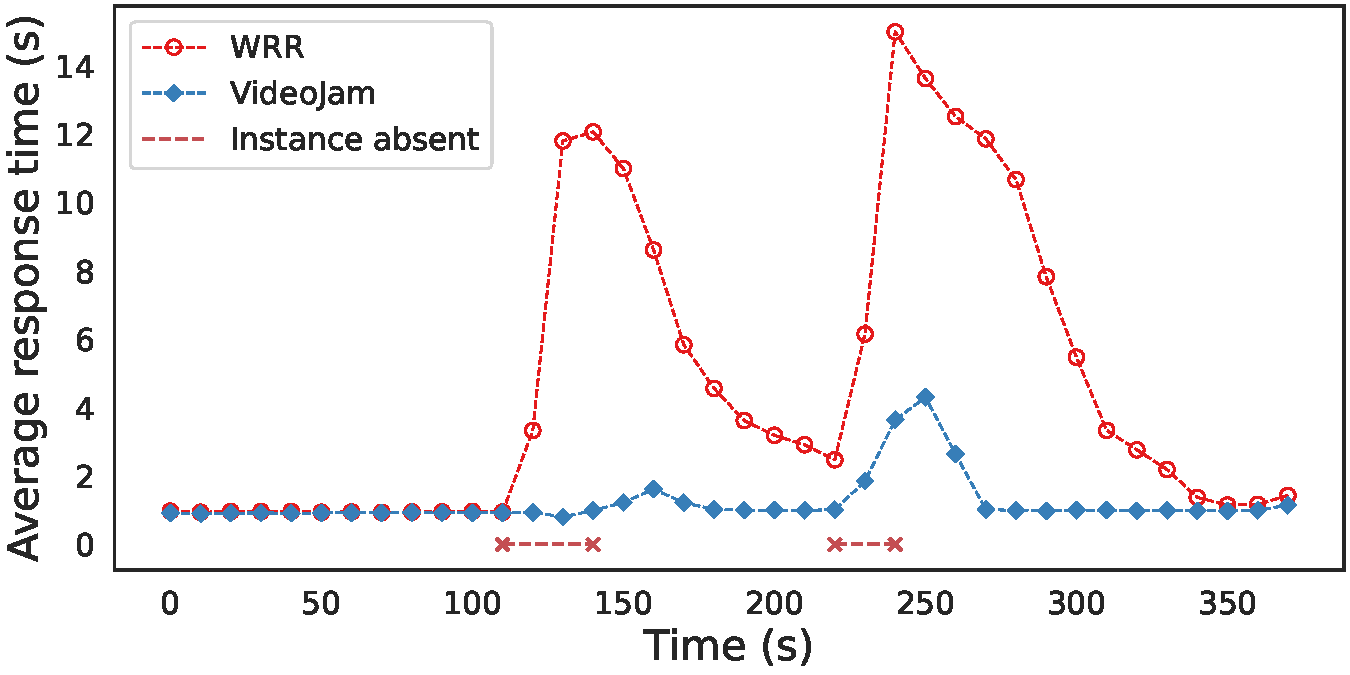
\includegraphics[width=\linewidth]{chapters/videojam/images/adaptability/average_response_time_timeseries.pdf}
		\subcaption{Averages for frames exiting YOLO.}\label{fig:adaptability_avg_response_time}
	\end{minipage}
	% \hfill
	\begin{minipage}[t]{.32\linewidth}
		\centering
		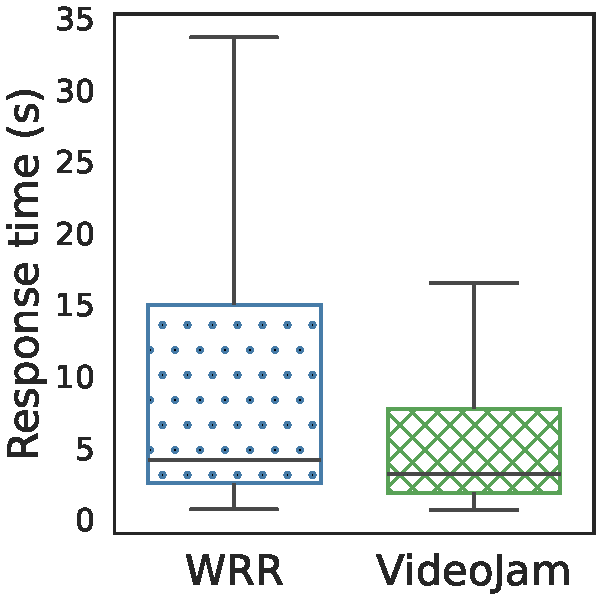
\includegraphics[width=\linewidth]{chapters/videojam/images/adaptability/response_time.pdf}
		\subcaption{Response time.}\label{fig:adaptability_response_time}
	\end{minipage}
	\vspace{-1mm}
	\caption{Evaluation under node failure conditions: WRR's poor performance and~\videojam{}'s adaptability under failures.}
	\vspace{-3mm}
	\label{fig:adaptability}
\end{figure}


\paragraph{\videojam{} Under Different Workloads.} To evaluate the sensitivity of~\videojam{} to the level of workload, we subject it to different workloads, increasing the number of source cameras given a fixed function placement (deployment). In this scenario, we use six \acrshort{gpu}-equipped nodes, and we set the number of YOLO and OCR instances to three and five respectively, while we increase the number of mobile cameras from two to five with a rate of 15 frames per second. 

~\Cref{fig:against_wrr} shows the system response time, the percentage of lost frames, and the bandwidth used during the offloading.~\videojam{} generally shows better performance with respect to the other compared solutions. The poor performance of no-balancing strategy highlights the need of load balancing solutions in this context. WRR reasonably shows longer response times as the load increases since such solution struggles in presence of network congestion. This is also highlighted by the increase in the bandwidth utilization showed in~\Cref{fig:against_wrr_bandwidth}.~\videojam{}, on the other hand, even in the event of congestion, only offloads the difference between instances to prevent two instances from sending load to each other, which explains the low bandwidth used. Furthermore, given the efficient collaboration among neighbors,~\videojam{} maintains stable performance as the workload increases.

In summary, this experiment has shown that~\videojam{} balances the workload without compromising performance, while minimizing system response time. In addition, while WRR statically balances incoming workload to neighbors,~\videojam{} adapts to the current situation by computing the most appropriate policy, and prevents bandwidth wastage due to bidirectional load migration.



\paragraph{\videojam{}'s Adaptation to Functions Placement.}
We evaluate the impact of different placement strategies (configurations) on~\videojam{}, particularly in the case of real-time variations. Note that there is a fundamental difference between workload variations and configuration changes or function placement strategies. Whereas in the previous experiment, we studied workload variation, which applies to the number of objects to be processed in each video stream, in this experiment we will study the case of configuration changes, which applies to the number of streams and processing modules available in the system.

Many studies have been carried out to find a better solution for placing components or functions to maximize the use of hardware resources while maintaining good precision~\cite{201465videostorm,hung2018videoedge}. As~\videojam{} is agnostic of the placement, we aim to evaluate if performance remains stable across different configurations. To do this, we start with four sources (15fps), three low-resolution YOLOs and five OCRs. First, we deliberately remove a YOLO function before redeploying it, but this time with a higher resolution, but with a higher inference time (lower throughput). This corresponds to a configuration change that can occur when placement techniques are used. In a second step, we kill all components (YOLO and OCR) on another node before restarting them after about 15 seconds. This simulates a node failure that can occur at any time when dealing with edges.

The system response time and the average response time of frames, as they leave the YOLO component, are shown in~\Cref{fig:adaptability_response_time} and~\Cref{fig:adaptability_avg_response_time} respectively. Initially, YOLOs maintain a consistently low response time, as they efficiently handle the incoming workload that is below their capabilities. At $\sim$100s (\Cref{fig:adaptability_avg_response_time}), a YOLO instance fails, with the source previously connected to it now sending its stream to another instance. This results in a sudden increase in the load that is badly distributed between instances for WRR. In contrast, in with~\videojam{}, instances remain capable of handling all the load generated by the sources. When the function is reintroduced into the system with a different configuration (higher resolution), WRR shows a gradual and slow decrease in response time, as it is unable to redistribute the loads already allocated to instances. 

\begin{figure}[t!]
	\centering
	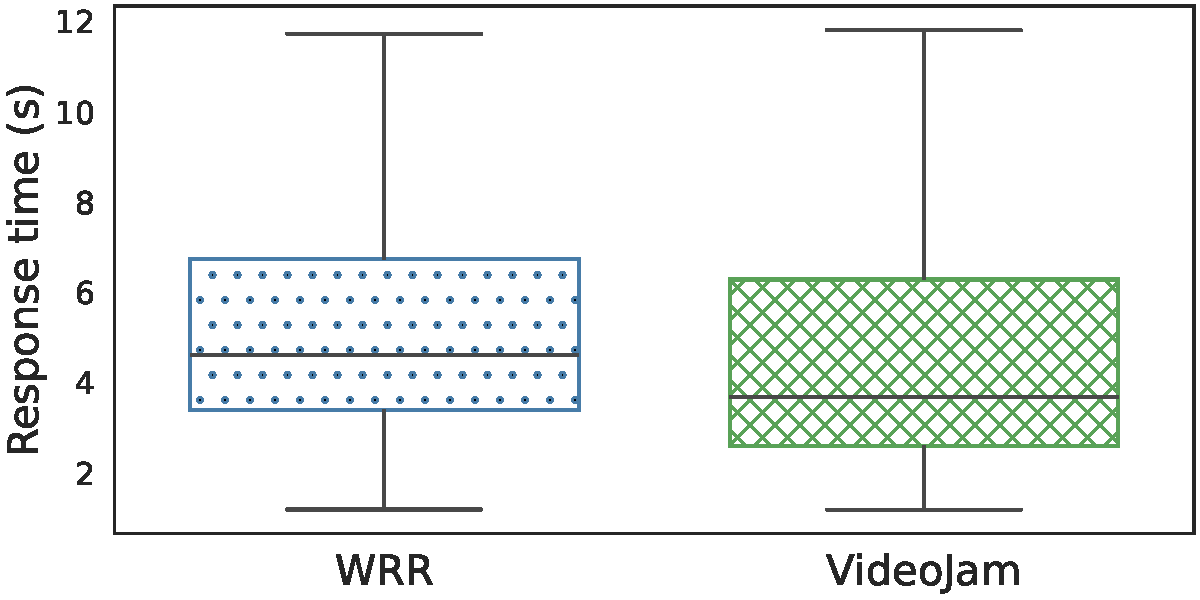
\includegraphics[width=.6\linewidth]{chapters/videojam/images/impact_of_mobility/response_time.pdf}
	\caption{Little effect of source mobility and abrupt flow changes on~\videojam{} performance.}
	\label{fig:impact_mobility}
\end{figure}

A similar behavior is observed at $\sim$220s, where a YOLO and an OCR deployed in the same node are killed due to node failure. Here again, the response time increases for WRR and~\videojam{}. In this particular case, the remaining YOLOs (one high-resolution and one low-resolution) are unable to handle the incoming workload, resulting in an increase in response time. In contrast,~\videojam{} excludes the outgoing instance from the load-balancing policy until it returns, or new functions are added, allowing previously accumulated overload to be efficiently redistributed between instances.


\paragraph{Impact of Mobility.} One of the key features of mobile cameras is their ability to be in the right place to retrieve useful information. We aim to emulate mobile cameras, such as dash cams mounted on cars, entering and leaving the system. We emulate this scenario in our experiment as follows: at first, we have a camera streaming mobile content (\ie, a dash cam content as described in~\Cref{sec:setup}, in the paragraph related to the datasets); after a fixed amount of time, the camera leaves the system, emulating the car leaving the area currently being processed. Finally, a new video starts streaming, emulating a new car entering the system. For the experiment, we used three moving cameras (20fps) which send their streams to four YOLOs, which in turn send them to five OCR instances. At a given time, one camera stops sending its stream to the next function for a short period of $\sim$15 seconds. This represents a camera leaving the system and has a direct impact on the load, as the incoming workload correlation is broken. We observe the system response time in~\Cref{fig:impact_mobility}. When a source stops sending its data stream to the next function, the latter sees its incoming load drop drastically and then fails~\videojam{}'s prediction. Even though WRR is agnostic to these events as it continues to distribute frames independently of sources,~\videojam{}'s load balancing compensates for eventual forecasting errors, maintaining 1.25$\times$ better response time.